\section{Results}\label{sec:3}

\subsection{Thirty-four of 1,014 authorising provisions are determinate bindings}\label{sec:3.1}

Across the corpus, 1,014 provisions authorise. The frozen predicate returns 91 of them as determinate bindings; 491 reach an evaluation without a determinate operator; and 432 reach none. The audit of Section 2.7 then separates the 91: 41 are bindings and 50 are not, a precision of 0.451; this is a census of the returned set, with a Wilson 95\% interval of [0.352, 0.553] and an instrument-clustered bootstrap interval of [0.306, 0.518] (Section 2.7).

Determinate binding is therefore the exception twice over. It is the exception among authorising provisions, at 4.0\% of the 1,014 after audit against 9.0\% before it, and the indeterminate case is the mode by an order of magnitude. And it is the exception among the provisions the predicate itself returns, nearly two thirds of which do not withstand reading. Both of those denominators are themselves audited: Section 2.8 measures the authorising population to be contaminated at 0.494, which raises the corpus-wide rate from 4.0\% to 8.2\% and raises it unevenly, so the rate is reported in both coordinates wherever it carries an argument.

Both numbers are reported throughout. The first states what a frozen, published rule returns and can be reproduced from the released files without reading a word of law; the second states what survives a reader, and is the number every substantive claim below rests on. Where they

differ the difference is reported, because the gap between them is itself a finding about what automated regulatory measurement can and cannot assert.

\subsection{Following cross-references does not reveal hidden bindings}\label{sec:3.2}

The central methodological claim of this design is that a binding is a property of a path rather than of a provision, and that reading provisions one at a time therefore understates how much technical binding a corpus contains. The audit allows that claim to be tested rather than asserted, because it separates the bindings the predicate finds into those that survive reading and those that do not. It does not survive the test.

Deleting every edge and asking only what each paragraph says on its own returns 72 provisions that satisfy the predicate. Thirty of them are audited bindings. Restoring the cross-reference graph raises the count to 91 and the audited bindings to 34. The graph therefore contributes four additional bindings and fifteen additional false positives (Table 7). Of the 41 audited bindings, 37 (90.2\%) are visible in a single paragraph read alone, and 4 (11.8\%) exist only because a reference is followed. The conclusion is unchanged in direction and weaker in degree: precision still falls monotonically as the bound is relaxed, from 0.417 on a single-paragraph reading to 0.451 at four hops, so following cross-references still costs more in false positives than it buys in bindings.

\begin{table}[!htb]
\centering
\caption{What the cross-reference graph adds. Each row applies the frozen predicate at a different path bound to the same 1,014 authorising provisions; the audit of Section 2.7 then separates the provisions it returns. Precision falls monotonically as the bound is relaxed.}
\label{tab:t7}
\small
\begin{tabular}{@{}lrrrr@{}}
\toprule
Condition & Audited bindings & False positives & Returned & Precision \\
\midrule
No edges (provision read alone) & 37 & 35 & 72 & 0.514 \\
hop $\le$ 1 & 37 & 39 & 76 & 0.487 \\
hop $\le$ 2 & 41 & 47 & 88 & 0.466 \\
hop $\le$ 3 & 41 & 49 & 90 & 0.456 \\
hop $\le$ 4 (adopted) & 41 & 50 & 91 & 0.451 \\
\bottomrule
\end{tabular}
\end{table}

The single binding that the graph does contribute is the one the design was built to catch. Article 5(1) of Regulation (EU) 2019/947 requires a UAS operator to obtain an operational authorisation pursuant to Article 12 where a requirement of Article 4 or Annex Part A is not met, and Article 12(1) is where the competent authority shall evaluate the risk assessment and the robustness of the proposed mitigating measures. The operator, the referral and the evaluation are written in three places, and only following the reference assembles them. That this structure exists is not in doubt. What the audit shows is that it is rare, and that the same traversal which finds it also manufactures 15 returns that are not bindings.

This runs against our own earlier reporting, and we state the correction plainly. An earlier, unsubmitted draft of this manuscript reported that 19 of 78 bindings, a quarter of the total, were invisible to provision-by-provision reading, and drew from that the methodological conclusion that provision-level audits systematically understate the hardest category. That figure was computed over unaudited counts. Once the counts are audited it inverts: the provisions that the graph adds are overwhelmingly provisions in which an authorisation and an evaluation word happen to lie within four hops of one another without the second conditioning the first. For this corpus, reading each authorising provision on its own is not a weaker instrument than following its references. It is a more precise one.

Two qualifications bound that conclusion. It is a statement about precision, not about recall: the audit samples only provisions the predicate returned, so it cannot say how many bindings a single-provision reading would miss, and the lexicon validation of Section 2.6 bears on that question instead. And it is a statement about this corpus, in which cross-references between a determinate operator and a named evaluation turn out to be uncommon; a corpus of framework statutes that delegate their technical content wholesale would not behave this way.

\subsection{What binds is the machine, and the pooled ground rate hides it}\label{sec:3.3}

The 41 audited bindings are not spread evenly across regulatory domains (Table 9). Aviation instruments convert 10.8\% of their authorising provisions into audited bindings. Ground-robot and road-traffic instruments convert 2.5\%. The cross-cutting instruments that govern data protection, artificial intelligence, measuring instruments and police equipment convert none at all. The aviation-to-ground ratio is 4.34, with Cohen's h = 0.353. Correcting both denominators for the contamination measured in Section 2.8 raises the two rates to 21.7\% and 4.5\% and the ratio to 4.8, because the contamination is heavier in aviation; the nominal pair is the conservative statement of the contrast and is the one quoted throughout.

Wilson 95\% intervals on the three nominal rates are [7.5, 15.3], [1.5, 4.1] and [0.0, 2.2] per cent, and those intervals assume provisions are independent. They are not, for the reason given next, and under the design effect measured there they widen to [4.9, 22.1], [0.9, 6.8] and [0.0, 9.6]. Both are reported in Table 9 and the wider pair is the one any comparison between domains has to use.

The unit of analysis is the instrument, not the provision. Earlier versions of this paper tested this contrast with a Fisher exact test over provisions and reported p = 1.5 $\times$ 10$-$6 with an odds ratio of 5.7. That test is withdrawn as a finding, and the reason is visible in the data it was run on. Bindings do not arise independently provision by provision; they arise where an instrument is drafted to condition permissions on technical evaluation, and then they arise in numbers inside that instrument. Of the 26 aviation bindings, 24 are in two instruments, 17 in Regulation (EU) 2018/1139 and 7 in 14 CFR Part 107, and two of the six aviation instruments contribute none. All 15 ground bindings are in four of the five ground instruments. The intraclass correlation of the binding indicator across the sixteen instruments is 0.067, which at an effective (Kish) cluster size of 56 provisions, against an arithmetic mean of 63 and a median of 34, gives a design effect of 4.68 and an effective sample size of 217 against a nominal 1,014. A provision-level test on this structure counts each instrument's drafting decision once per provision, which is pseudoreplication, and it is the error this paper is otherwise about.

Taking the instrument as the unit, the contrast does not reach conventional significance and we say so plainly. There are six aviation instruments and five ground instruments. Relabelling them across the two domains gives 462 partitions, and the observed difference in pooled rates is equalled or exceeded in 41 of them: p = 0.09. A Mann-Whitney test on the eleven instrumentlevel rates gives p = 0.52. A design-effect correction applied to the provision-level table gives p = 0.018, but that correction treats the design effect as if it were a known constant and we do not rest on it. With six instruments against five, no test on this corpus has the power to separate the domains; the corpus is too small in its own unit of analysis, and that is a property of the available law rather than of the measurement.

What survives is therefore descriptive and we state it as such. Aviation instruments carry audited bindings at about five times the rate of ground instruments, the direction is the same in every instrument-level comparison, and the concentration in Regulation (EU) 2018/1139 and

Part 107 is the substantive observation: the contrast is between drafting traditions of particular instruments, not between two populations of provisions that a test could separate. Cohen's h = 0.353 sits in the range conventionally read as a small effect, and that is consistent with a large ratio between two small proportions, which is what h is designed to discount. Both effect measures carry intervals and we give them, because a ratio reported without one invites the reading the previous sentence warns against. On provision-level standard errors the ratio runs [2.34, 8.06] and h runs [0.20, 0.50]; under the design effect of 4.68 they run [1.14, 16.53] and [0.03, 0.68]. The corrected interval on the ratio excludes 1, and an earlier version of this paragraph called that the one inferential statement about domains this corpus supports. It is not, and the reason is the one the paragraph above gives for setting the corrected Fisher test aside: both treat the design effect as a known constant when it is estimated from the 16 instruments of the corpus. Held to that standard the interval does not survive. The design effect at which the lower bound reaches 1 is 5.65 against the 4.68 measured, so a 21 per cent movement in the design effect removes the exclusion. Dropping any one of four instruments (Regulation 2018/1139, 14 CFR Part 107, the Japanese Road Traffic Act, the Korean Road Traffic Act Enforcement Rule) removes it outright. Resampling with replacement the 11 instruments that contribute to the ratio, and recomputing the design effect in each draw, the corrected interval includes 1 in 53 per cent of the 9,864 draws in which the ratio is defined (136 of 10,000 draws lose one domain's bindings entirely and are discarded), with the design effect itself running [1.00, 8.23], where 955 draws return a negative variance-component estimate and are floored at 1. An earlier version resampled all sixteen instruments, including the five that contribute nothing to the ratio, and reported 54 per cent of 10,000; the figure here is both the one the released script computes and the less favourable of the two. We therefore make no inferential claim about domains. What the corpus supports is the ordering and the census, and a reader who concludes from the ratio that aviation law densely conditions authorisation on technical evaluation has read more into it than the figure carries.

The carve-out comparison in Section 3.4 is not affected by any of this. It is a census of one population of provisions under two bodies of law, with the corpus, the predicate and the labels held constant, so it requires no test and no independence assumption; what it reports is what the deletion removes, not an inference from a sample.

That is as far as the pre-registered partition goes, and it is not far enough, because the ground category is not one body of law. Of its 604 authorising provisions, 574 are road-traffic instruments that regulate human drivers and only 30 are the Korean robot instruments. Those two have no reason to behave alike, and they do not. We therefore repartitioned the same 41 audited bindings by subject matter, after seeing the composition of the ground corpus and before writing this paragraph, and report it as the post-hoc analysis it is (Table 8).

This partition is subject to the same objection as the pre-registered one, and for the same reason: its cells are instruments, and provisions inside an instrument are not exchangeable. We therefore report it descriptively and give the provision-level tests only as the quantity a reader would otherwise compute, labelled as what they are. Aviation certification carries bindings at a higher rate than road-traffic law, 26 of 241 against 14 of 574, and a provision-level Fisher exact test on that table gives p = 2.6 $\times$ 10$-$6 with an odds ratio of 4.8; against horizontal product law, 26 of 241 against 0 of 139, it gives p = 6.7 $\times$ 10$-$6 , and against the pooled cross-cutting denominator p = 9.3 $\times$ 10$-$7 . None of these is offered as a tested finding. Each is computed over provisions, the design effect of the instrument clustering is 4.68, and the two aviation bindings outside Regulation (EU) 2018/1139 and Part 107 are what any instrument-level test would have to work with.

An earlier version of this paper declined one of these comparisons on the ground that a cell holding no events carries no test, while performing another that pools the same cell with a smaller

\begin{table}[!htb]
\centering
\caption{The same 41 audited bindings repartitioned by subject matter. This partition is post-hoc: it was made after the composition of the ground corpus was seen, and it is reported because the pre-registered partition pools instruments that do not behave alike. Rates are audited bindings over authorising provisions, with Wilson 95\% intervals. The instrument counts in parentheses are: aviation certification is Regulations 2018/1139, 2019/947 and 2019/945, 14 CFR Parts 107 and 89 and AC 00-1.1B; robot certification is the Korean intelligent robots act and its decree; road traffic is the Japanese and Korean road traffic instruments; police conduct is the Law Enforcement Directive, the Seattle ordinance and the California code; horizontal product law is the AI Act and the Measuring Instruments Directive.}
\label{tab:t8}
\small
\begin{tabular}{@{}lrrrrr@{}}
\toprule
Subject & Auth. & Audited & Rate & Wilson 95\% CI & Design-effect 95\% CI \\
\midrule
Aviation certification (6) & 241 & 26 & 10.8\% & [7.5, 15.3] & [4.9, 22.1] \\
Robot certification (2) & 30 & 1 & 3.3\% & [0.6, 16.7] & [0.2, 41.5] \\
Road traffic, drivers (3) & 574 & 14 & 2.4\% & [1.5, 4.1] & [0.8, 6.9] \\
Police conduct (3) & 30 & 0 & 0.0\% & [0.0, 11.4] & [0.0, 37.5] \\
Horizontal product law (2) & 139 & 0 & 0.0\% & [0.0, 2.7] & [0.0, 11.5] \\
\bottomrule
\end{tabular}
\end{table}

one. The stated criterion was wrong: power depends on the denominator rather than on the count in the empty cell, and applying it inconsistently withheld a quantity while reporting its pooled cousin. We correct it here, and the correction promotes nothing, because the unit of analysis defeats every number in this table equally. The small-cell comparisons show the same thing from the other end. Robot certification returns 2 of 30, with a Wilson interval of [1.8, 21.3] per cent wide enough to contain both the aviation and the road-traffic rate, so the failure of a provision-level Fisher test to separate it from aviation (p = 1.00) is an absence of power and not a finding of equivalence. The police-conduct instruments return 0 of 30 and are not separable from the aviation rate either (p = 0.088).

The two zero cells deserve a sentence of their own, because the design effect changes what they support. On provision-level Wilson intervals, horizontal product law at 0 of 139 has an upper bound of 2.7 per cent, which sits below the aviation rate of 10.8 per cent, and the crosscutting denominator at 0 of 169 has an upper bound of 2.2 per cent; read that way, each excludes the aviation rate. Under the design effect of 4.68 the bounds move to 11.5 and 9.6 per cent and neither excludes it. We had leaned on the first of these as the quantitative support for treating horizontal product law as a different regime from aviation certification, and on the corrected interval it does not carry that weight. What the table supports is an ordering of instruments by rate, with the two densest instruments identified, and not a claim that the categories differ.

What the repartition establishes is therefore negative and it is about our own pre-registered partition rather than about the law. The pooled ground rate of 2.5\% is produced by a denominator that is 95\% human driver licensing, so it cannot be read as a statement about ground robotics, and the pooled cross-cutting zero is carried by the AI Act and the metrology Directive, which supply 139 of the 169 provisions while the instruments that actually regulate police conduct supply 30. Both pooled figures appear in Table 9 and in our earlier drafting, and both should be read as descriptions of a mixed denominator. The statements this paper rests on about police-conduct instruments and about the Korean robot statute are readings of their text, set out in Sections 4.4 and 3.4, not statistical contrasts.

The objects the aviation bindings attach to are worth stating precisely, and we measured them rather than asserting them. Each of the 41 audited bindings was classified, in two passes over its own text carried out the same way as the binding audit of Section 2.7 and subject to the same caveat, by which permission it conditions: permission to supply the artefact (design, produce, type-certify, place on the market) or permission to operate it (fly, drive, conduct an operation,

\begin{table}[!htb]
\centering
\caption{Bindings by regulatory domain, before and after audit. No analyst-written search terms enter the returned column; it is computed from the lexicons and the graph over all authorising provisions. The audited column applies the labels of Section 2.7. Precision differs by a factor of nearly two between aviation and the ground corpus and is zero across the cross-cutting instruments, so the returned counts are not comparable between domains and the audited counts are. Aviation is Regulations 2018/1139, 2019/947 and 2019/945, 14 CFR Parts 107 and 89, and AC 00-1.1B; ground is the Japanese and Korean road traffic instruments and the Korean intelligent robots instruments; cross-cutting is the AI Act, the Measuring Instruments Directive, the Law Enforcement Directive, the Seattle ordinance and the California code.}
\label{tab:t9}
\small
\begin{tabular}{@{}lrrrrrr@{}}
\toprule
Domain & Auth. & Ret. & Aud. & Rate & Design-effect 95\% CI & Precision \\
\midrule
Aviation (6 instruments) & 241 & 54 & 26 & 10.8\% & [4.9, 22.1] & 0.481 \\
Ground (5 instruments) & 604 & 34 & 15 & 2.5\% & [0.9, 6.8] & 0.441 \\
Cross-cutting (5 instruments) & 169 & 3 & 0 & 0.0\% & [0.0, 9.6] & 0.000 \\
Total & 1,014 & 91 & 41 & 4.0\% &  & 0.451 \\
\bottomrule
\end{tabular}
\end{table}

use a facility). The passes agreed on all 41, including on the single provision each recorded as borderline; as there, the figure measures repeatability of a procedure, not agreement between two readers. The borderline record was resolved against the provision text by the procedure of Section 2.7.

Thirty-five of the 41 bindings condition operating, not supplying. Within aviation the split is 20 operating to 6 supplying, and every one of the 15 ground-side bindings conditions operating: 14 are driving licences and the fifteenth is the Korean robot change-certification provision. All six supply-side bindings are the classical ones and all six are in Regulation (EU) 2018/1139: type certification of a design, certification of parts and of non-installed equipment, the airworthiness certificate of an individual aircraft, certification of design and production organisations, and the certificate for a flight simulation training device. Two corrections to the earlier version of this paragraph belong here, because both were errors of identification rather than of counting. It listed certification of ATM/ANS systems and constituents as a seventh supply-side binding; the re-adjudication rejects Article 45(2) of the basic act, because the same paragraph permits the organisation to declare compliance instead of holding a certificate, and a branch that reaches the permission without the evaluation fails the rule. It also listed an eighth supply-side binding described as Article 40-2(3) of the Korean Intelligent Robots Act barring use of a robot inside a development district before completion certification. That description belongs to Article 37(4), which bars the project implementer from using land and facilities before the completion certificate and is not a binding under the audit; Article 40-2(3) is a duty to obtain change certification when altering certified matters, and because the certification it alters is the outdoor mobile robot operating-safety certification it conditions operating rather than supply. The twenty operating-side aviation bindings are pilot and air traffic controller licences, cabin crew attestations, training organisation and aero-medical centre approvals, instructor and examiner certificates, aerodrome certificates, air operator certification, the UAS operational authorisation of Implementing Regulation (EU) 2019/947, and the United States small unmanned aircraft operating rules of 14 CFR Parts 107 and 89.

An earlier version of this paper stated that nineteen of the aviation bindings bind the machine as an article of commerce and that 14 CFR \S{}89.110(b) is the only one conditioning flying rather than selling. The measurement says close to the opposite, and we report the correction rather than the claim. What distinguishes \S{}89.110(b) is not that it conditions operating, which most of them do, but that it is the only one of the 23 aviation bindings that survives the police carve-out (Section 3.4).

The ground figure is carried by two national road-traffic regimes. Of the 15 ground bindings, 5 are in the Korean Road Traffic Act and condition a driving licence on passing the driving examination or, for an existing holder, on undergoing a periodic aptitude test. The remaining 2 are in the Korean Intelligent Robots Act: one requires re-certification when a certified matter changes, and the other prohibits use of a development site before a completion certificate is issued. The remaining 4 are in the Japanese Road Traffic Act and are discussed below. Only the Korean re-certification provision is about a robot at all, and it is the only provision in the entire ground corpus where a robot's certified condition determinately conditions a legal right. The other 9 condition a human driver's licence on a human driver's examination.

The Japanese Road Traffic Act contributes 8 of the 41 bindings, and the history of that number is the clearest evidence we have that the instrument was asymmetric before it was symmetric. An earlier version of this paper reported a Japanese zero and read it as a false negative of the measurement rather than an absence in the law, naming the cause correctly, that the Japanese lexicon lacked the term the Act uses for the driving examination where the Korean lexicon carried its cognate, and declining to repair it because the ruleset had been frozen. The tier-0 sample described in Section 2.10 forced the issue: the omission was not one term but a class of them, so we symmetrised the lexicons in both directions and re-ran. The Act now returns 20 provisions and the audit accepts 4. Article 89(1) conditions the grant of a licence on sitting the examination the public safety commission conducts, and Article 104-2-2(1), (2) and (4) require the commission to revoke a licence where the holder fails the re-examination or does not sit it. The 16 rejected are reporting duties, validity-period tables, eligibility restrictions and discretionary refusals, in which an evaluation term appears as a date, as a description of who is examined, or alongside a power the commission may exercise rather than one it must.

What the Japanese four are is as important as that they exist. They condition a human driver's licence on a human driver's examination. They are not a machine certified against a stated threshold, and they enter the ground denominator that Section 3.3 already discounts as humandriver licensing. Their arrival moves the ground rate from 1.2 to 1.8 per cent and the aviation-toground ratio from 8.07 to 5.13 without moving anything on the police route; the ratio reaches its current 4.34 only after the paragraph test of Section 2.10 takes the aviation denominator from 246 to 241. An earlier version of this sentence attributed the whole move to the Japanese provisions and still printed the later endpoint.

The cross-cutting figure is the one that bears on police conduct most directly, and after audit it is 0 of 169. The Law Enforcement Directive contributes 14 authorising provisions and no binding before or after audit; the two police-equipment governance instruments contribute 16 and none. The AI Act contributed two returned provisions and the Measuring Instruments Directive one, and the audit rejected all three: a high-risk classification rule, a transitional application rule, and a market-access provision whose only evaluation term lies in a definition list. These instruments are determinate about purpose, authority and process, and silent about the technical performance on which the authorised act depends.

\subsection{The police carve-out leaves one audited binding, and it is about the aircraft's own position}\label{sec:3.4}

The aerial mission was adjudicated twice against the same corpus and rule, once on the civil route and once with the carve-out applied as a deletion of 1,164 nodes (Fig. 3).

On the civil route the predicate returns 54 provisions, of which 26 survive the audit. On the police route it returns 7, of which one survives. The carve-out therefore removes 25 of the 26 audited technical bindings that a civil unmanned aircraft carries, 96 per cent of them, and leaves one. On the returned counts the figure is 47 of 54, or 87 per cent.

An earlier version of this paper reported that total as 19 of 19 and stated that no audited binding survives. We were wrong, and the error lay in the measurement rather than in the reading: the determinacy lexicon was suppressing the construction may . . . only if throughout the English material, for the reason set out in Section 2.10. Correcting it returns 14 CFR \S{}89.110(b), which the audit confirms as a binding and which the carve-out does not touch. We report the survivor first and in full, because it is the provision that comes closest to refuting this paper.

What the surviving binding binds. Section 89.110(b) provides that a person may operate a standard remote identification unmanned aircraft only if its serial number is listed on an FAAaccepted declaration of compliance, or the aircraft is covered by a design or production approval and meets the requirements of Subpart F. The operator is the authorising modal, the determinate

\begin{figure*}[!t]
\centering
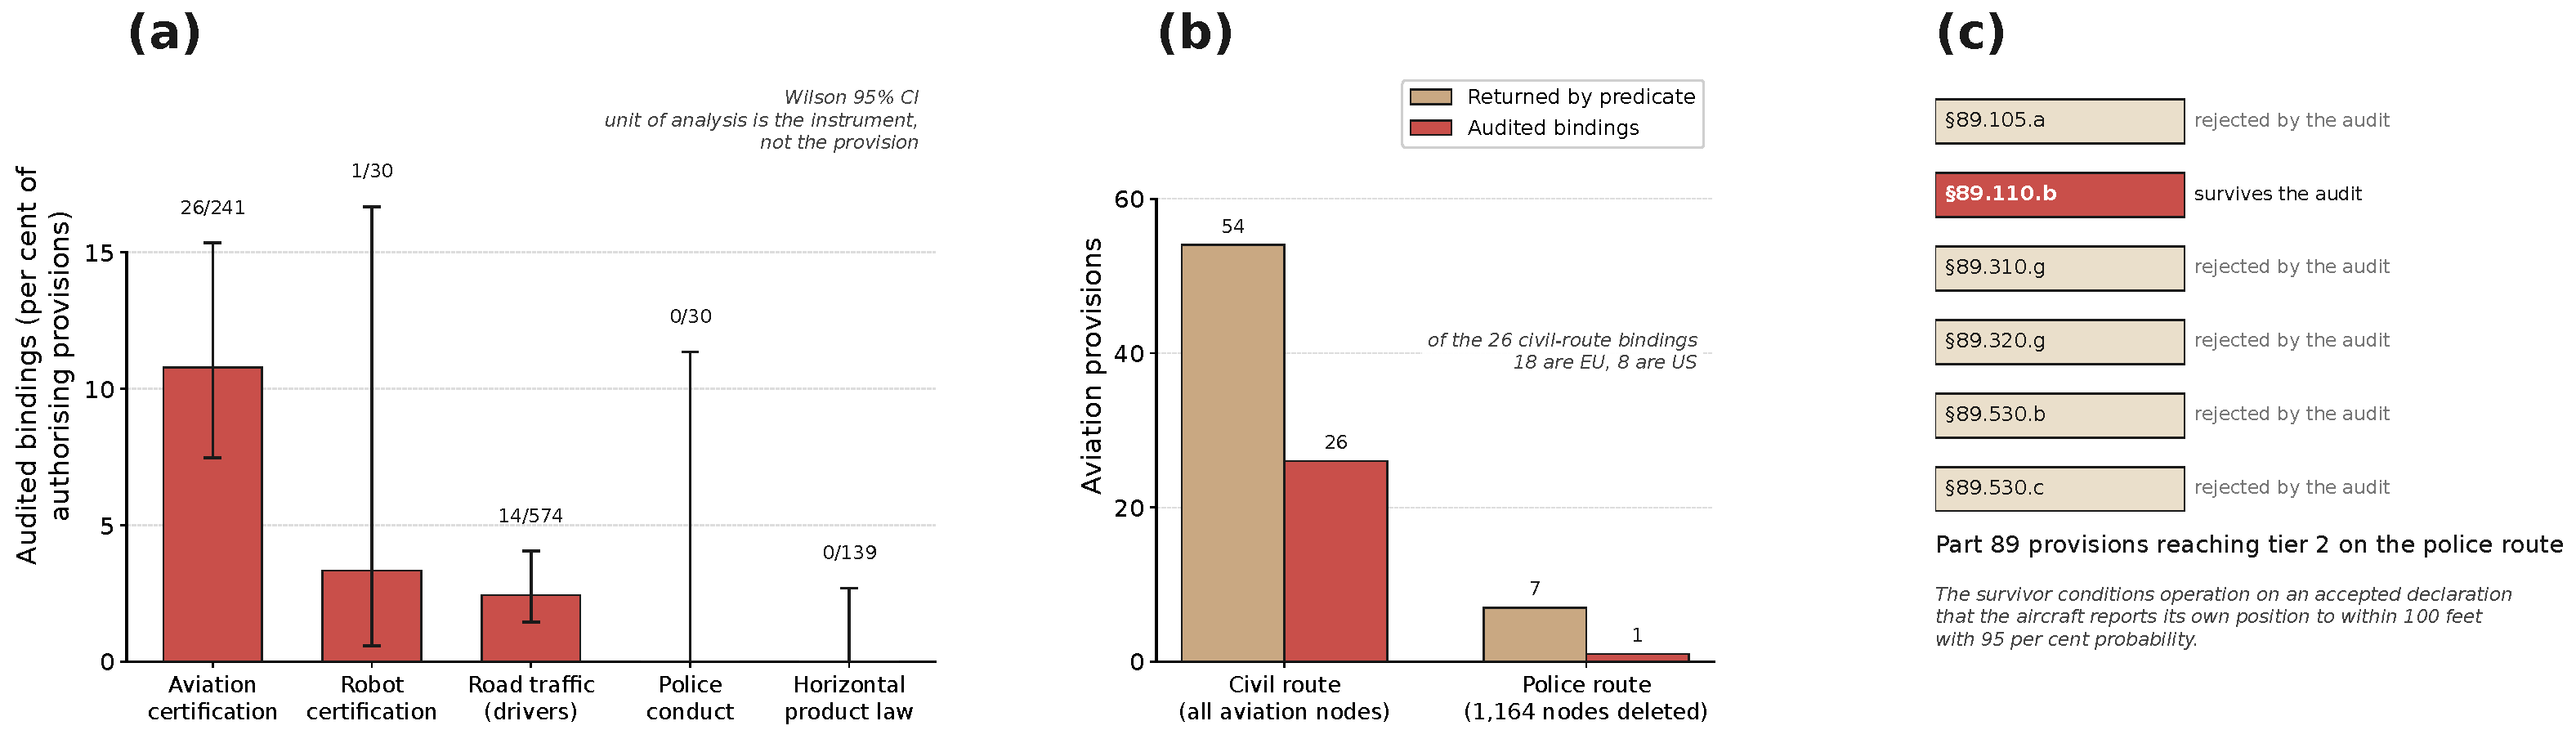
\includegraphics[width=\textwidth]{FigR}
\caption{Where audited bindings are, and what a police exemption removes. (a) Audited bindings as a share of authorising provisions, by subject matter, with Wilson 95\% intervals and the count over the total above each bar. The partition is the post-hoc one of Table 8. The rates are descriptive: the unit of analysis is the instrument, not the provision, and at instrument level the domains do not separate, so the panel carries the clustering statistics rather than a test (Section 3.3). The two cells of 30 provisions are shown for composition. (b) The same airframe adjudicated on the civil route and with the police and public-aircraft carve-outs applied as deletions of 1,164 of the 5,758 nodes in the provision graph, everything else held constant; the returned counts are 54 and 7, the audited counts 26 and 1. Of the 26 civil-route bindings, 18 are EU and 8 are US; the EU deletion removes all 1,047 nodes of the three EU instruments, while the US deletion is selective and leaves 306 aviation nodes holding 34 authorising provisions in force, among which one binds. (c) What the exemption leaves. 6 provisions of Part 89 reach tier 2 on the police route and one, \S{}89.110(b), survives the audit: it conditions operating a standard remote identification unmanned aircraft on an accepted declaration that the aircraft reports its own position to within 100 feet with 95 per cent probability. Part 89 was made in 2021, after the public-aircraft doctrine was settled, and is not among the instruments AC 00-1.1B exempts.}
\label{fig:f3}
\end{figure*}

operator is only if, and the object of the condition is a named evaluation named in the same paragraph. It satisfies all three audit conditions, and it survives the disjunction test of Section 2.7: requirement (b)(2) independently demands that the aircraft's remote identification equipment be functional and comply with this part, and \S{}89.125 bars ADS-B Out from being used to comply with the remote identification requirements of this part, so the one branch of (b)(1) that would otherwise bypass \S{}89.310 is closed by a requirement conjunctive with it.

The content of that declaration is fixed four provisions away, and the chain is worth setting out because the content of the evaluation is the whole of the finding. Section 89.530(a) requires the producer of a standard remote identification unmanned aircraft under \S{}89.515 to submit a declaration of compliance for FAA acceptance. Section 89.515(a) requires such an aircraft to be designed and produced to meet the minimum performance requirements established in \S{}89.310. And \S{}89.310(h)(1) requires that the reported geometric position of the unmanned aircraft and the control station be accurate to within 100 feet of the true position, with 95 percent probability. The alternative branch of \S{}89.110(b)(1), a part 21 design or production approval plus the requirements of Subpart F, runs through \S{}89.510(b)(1) to the same section, but \S{}89.510(b) is itself disjunctive and its branch (2) is satisfied by ADS-B Out equipment meeting \S{}91.225, which reaches no evaluation. That branch is closed not by requirement (1) but by requirement (2) of \S{}89.110(b), which demands independently that the aircraft's remote identification equipment be functional and comply with this part, read with \S{}89.125, which provides that ADS-B Out equipment cannot be used to comply with the remote identification requirements of this part. We set the reasoning out because the audit split on it, one pass labelling the provision a binding and one not, and because \S{}91.225 lies outside the corpus so we cannot say from the measured text whether it names an evaluation of its own.

So where a police unmanned aircraft is operated as a standard remote identification unmanned aircraft, the permission is conditioned on how accurately it reports where it is. It is not the only route. Section 89.105 makes \S{}89.110 one of three ways to comply, the others being a broadcast module under \S{}89.115(a), which reaches the same kind of declaration through \S{}89.320, and operation inside an FAA-recognized identification area under \S{}89.115(b), which requires no remote identification equipment and no evaluation at all; \S{}89.105 also opens with an exception for operations the Administrator otherwise authorises. An earlier version of this paper called \S{}89.110(b) the authorisation a police unmanned aircraft must earn, which overstates it. What the measurement supports is that \S{}89.110(b) is the only binding in force on the police route, not that every police operation must pass through it.

Two things must be said about that chain. The first is that it is a reading of the text and not a measured path: the provision graph holds no edge from \S{}89.110(b) to \S{}89.310(h), because \S{}89.110(b) names the declaration of compliance as a term rather than as a numbered crossreference, and the predicate scored the provision tier 2 on the evaluation term in its own paragraph. We verified each link of the chain against the corpus text and release the check; we do not claim the graph found it. The second is what the threshold is about. One hundred feet at 95 per cent probability is a requirement on the broadcast position of the airframe. It says nothing about the accuracy of a chemical identification, a thermal reading, a face match or any other sensing on which a police decision might rest. The corpus contains no provision in force on the police route that conditions an authorisation on an evaluation of that kind, and the sweep of Section 3.5 is the independent check on that statement.

How the total is composed. Without this, the 25 reads as stronger than it is. The EU and US carve-outs are not the same kind of operation, and the 25 is a sum across two bodies of law that

no single aircraft is subject to at once. Split by jurisdiction, the EU side contributes 18 audited bindings on the civil route and 0 on the police route, and the deletion there removes all 1,047 nodes of Regulations 2018/1139, 2019/947 and 2019/945, leaving nothing of the EU aviation corpus behind. That is close to analytic: Article 2(3)(a) excludes police activities from the basic act, so the acts resting on it go with it, and a binding cannot survive in a text that is no longer in scope. The US side contributes 8 audited bindings on the civil route and 1 on the police route, and there the deletion is selective. It removes Subparts C and D of Part 107 and leaves 306 aviation nodes standing: the rest of Part 107, the whole of Part 89 and the advisory circular itself. The one surviving binding is in those 306 nodes. The informative measurement is there, not in the EU column, and we report the two separately for that reason.

The retained population. Three facts about the remainder are needed before any null is read. The first is its size in the paper's own unit. The 306 retained aviation nodes contain 34 authorising provisions, 17 in Part 89, 12 in the retained subparts of Part 107 and 5 in the advisory circular; the police route as a whole retains 807 authorising provisions of the 1,014, because the carve-out touches only the aviation instruments. Node counts and provision counts are not interchangeable and we give both.

Two of those three components are retained on grounds that do not hold, and the direction of the error matters. Part 107 applies, by \S{}107.1(a), to civil small unmanned aircraft systems, and 49 U.S.C. \S{}40102(a)(16) defines a civil aircraft as an aircraft other than a public aircraft; AC 00-1.1B says in terms that regulations whose applicability uses the phrase civil aircraft do not apply to public aircraft operations. On that reading the whole of Part 107 leaves the police route, not merely Subparts C and D, and the 12 retained Part 107 provisions go with it. The five advisory-circular provisions should not be in the authorising population at all: Section 2.3 declares guidance excluded and retains AC 00-1.1B only as the documentary basis for the carveout rule, and their presence is a failure to execute that exclusion, which we report rather than repair after the fact. The defensible retained population is therefore Part 89 alone, 17 authorising provisions, and the surviving binding is in it.

Every one of these choices was made in the direction that retains, which makes the police route look better covered than it is. Correcting them shrinks the retained population and leaves the result unchanged: the single surviving binding is in Part 89, which no one disputes remains applicable. Removing the five advisory-circular provisions also moves the nominal aviation rate from 10.8 per cent to 11.0 per cent, 26 of 236, which no conclusion turns on.

The second is the tier distribution of Part 89, which is where a counterexample would have to live, since Part 89 is the one aviation instrument the carve-out leaves entirely intact. Of its 17 authorising provisions, 6 reach tier 2: \S{}89.110(b), which is the binding, and five the audit rejects. Those five are \S{}89.105(a), which fails the disjunction test because its condition is satisfied by operating inside an FAA-recognized identification area under \S{}89.115(b) with no remote identification equipment and therefore no evaluation; \S{}\S{} 89.310(g) and 89.320(g), where the only evaluation term is a date reference, naming the date a declaration of compliance is submitted; and \S{}\S{} 89.530(b) and (c), which impose a declaration duty on a producer and list the information the declaration must carry. Two reach tier 1 and 9 reach tier 0. The two at tier 1 are \S{}89.115(a) and \S{}89.505(a). Two earlier versions of this distribution were wrong and both are reported in Section 2.10. The first listed \S{}89.530(i) at tier 1; no such provision exists in 14 CFR, and the entry was an artefact of the extraction defect that promoted \S{}89.530(c)(7)(i) to a top-level paragraph. The second, published through the eighth review round, gave the population as 20 and named four tier-1 provisions, two of which, \S{}\S{} 89.510 and 89.515, are section captions with paragraph children and were in the population only because the paragraph-node rule was not being enforced on United States identifiers. They reach a named evaluation through the same declaration-of-compliance chain as the binding and fail the predicate on the operator rather than on the evaluation: the obligation in each is on the producer, and the operating rule refers to equipment already produced under an accepted declaration without itself conditioning a grant of permission on an outcome. Section 89.110(b) differs from them in exactly one respect, which is that it addresses the operator and conditions the operation. We report the whole distribution rather than only the returns, because a reader checking the defeater of Section 2.10 should not have to take it on trust that nothing else in Part 89 reaches tier 2.

The third is recall on this population, and it is the weakest part of the paper. The lexicon projection of Section 2.6 gives a false-negative rate within a tier-1 population, and recall follows from it only if the audited bindings in the numerator and the tier-1 provisions in the denominator are drawn from the same population. Two earlier versions of this paper failed that condition in opposite directions and both are withdrawn. The first reported a recall of 88.6 per cent, which is one minus the false-negative rate and is not recall at all. The second divided one audited binding, which is the aviation survivor, by a projection taken over the whole police route, and reported the result as a recall of 1 in 43; the numerator was aviation and the denominator was not.

Matched populations give the following. On the police route as a whole there are 16 audited bindings and 367 tier-1 provisions, so the projection is 46 missed bindings with an interval of 17 to 108 and recall is 0.26 [0.13, 0.48]. On the aviation part of the police route, which is where the surviving binding and the negative claim both sit, there is 1 audited binding and 10 tier-1 provisions, the projection is 1.3 [0.5, 2.9] and recall is 0.44 [0.25, 0.68] on a population too small to carry weight. Corpus-wide, 41 audited bindings against 491 tier-1 provisions give a projection of 62 [23, 145] and recall 0.40 [0.22, 0.64]. The corrected figures are better for this paper than the withdrawn 1 in 43 by roughly an order of magnitude, which is the direction that obliges us to state plainly that the error was ours and that it understated our own instrument. The negative claim this paper makes is therefore bounded accordingly: what the measurement establishes is that the only binding the predicate can see on the police route conditions the aircraft's report of its own position, and that the predicate's recall on that population is low enough that the claim must be read as a statement about what a frozen, published, audited rule finds rather than as a census of the law.

\subsection{The legal form that would bind sensing performance exists and enumerates its scope}\label{sec:3.5}

Directive 2014/32/EU is the European legal-metrology regime, and it does, on its face, exactly what this paper has been asking whether any instrument does. We set out that reading before qualifying it, because the qualification matters: the provision in question is one of the 57 the audit rejected, and what follows is therefore a legal reading of the Directive, not a measurement of it. Article 7(2) requires Member States to take all appropriate measures to ensure that measuring instruments are made available on the market and/or put into use only if they satisfy the requirements of the Directive, and Annex I states that the error of measurement shall not exceed the maximum permissible error laid down in the instrument-specific requirements. A permission is conditioned determinately on a stated metrological performance.

Article 2(1) then enumerates what the Directive applies to: water meters (MI-001), gas meters and volume conversion devices (MI-002), active electrical energy meters (MI-003), thermal energy meters (MI-004), measuring systems for continuous and dynamic measurement of liquids other than water (MI-005), automatic weighing instruments (MI-006), taximeters (MI-007),

material measures (MI-008), dimensional measuring instruments (MI-009) and exhaust gas analysers (MI-010).

No category is a law-enforcement measuring instrument. No category is a chemical, biological, radiological or nuclear detector, an airborne sensing payload, or any instrument whose reading supports a police determination. The form that would close the gap is neither missing nor immature. It has existed in its present shape since 2014 and in its predecessor since 2004, and its scope was drawn by enumeration.

Two qualifications are owed on this subsection, and both run against us. The first is the one stated above: Article 7(2) is a provision the audit rejected. The predicate reached its evaluation term in the definitions of Article 4 rather than in Annex I, and the chain drawn in Fig. 4a is the chain a lawyer reads, not the path the predicate recorded; with the unnumbered structural edges removed the provision falls to tier 0. We had described this instrument as a positive control demonstrating that the predicate finds the structure when it is present, and that description does not hold. A third point runs the same way and is owed to the reading above. Article 7(2) obliges Member States to take all appropriate measures to ensure that instruments are made available or put into use only if they satisfy the Directive, and that is the same form of qualification the next subsection uses to reject AI Act Article 15. The hedge list of Section 2.6 carries as appropriate and where appropriate but not this phrase, so the predicate did not treat it as a hedge. Adding the phrase to that list is a one-line change whose measured effect is to move Article 7(2) to tier 1 and the returned count from 91 to 90, leaving the audited bindings unchanged. We report the omission rather than repair it after the fact, and note that the repair would remove the only provision this subsection discusses from the returned set altogether. The second is that Article 3, headed Optionality, provides in paragraph 1 that Member States may prescribe the use of measuring instruments for measuring tasks where they consider it justified for reasons including public safety and public order, so Article 2(1) enumerates the categories for which Union-level requirements exist rather than the whole set of instruments subject to legal metrology. The enumeration is a boundary of competence as much as a boundary of legislative attention, and the Korean Measurement Act we were unable to retrieve belongs to precisely the national layer this qualification points at.

\subsection{The closest thing to a counterexample, and why it is not one}\label{sec:3.6}

A negative result is only as good as the search that failed to refute it, and the lexicon projection of Section 2.6 bounds how many bindings of any kind the predicate misses without saying whether a missed one would concern sensing performance. We therefore ran a second search that does not use the predicate at all. Seventeen concepts of measurement and sensing performance were matched against the text of all 5,758 provision nodes: maximum permissible error, measurement error, accuracy, precision, detection limit, false positive and false negative rate, sensitivity, specificity, calibration, metrology, tolerance, uncertainty, repeatability, reproducibility, resolution, a stated performance standard, and the construction within n feet, metres or seconds. Each concept is expressed in all three languages of the corpus, and the search script asserts that before it runs, so a concept cannot be present in English and absent in Korean or Japanese. The seventeen concepts expand to 78 patterns, 23 English, 30 Korean and 25 Japanese, matched on word stems rather than exact forms.

Two changes widened this sweep and both are reported. An earlier version matched whole words and therefore missed accurate where it had looked for accuracy. A later version, the one reported through the eighth review round, had stemmed the English entries but left the Korean and Japanese entries as bare nouns, so no Korean or Japanese node matched at all and the

\begin{figure*}[!t]
\centering
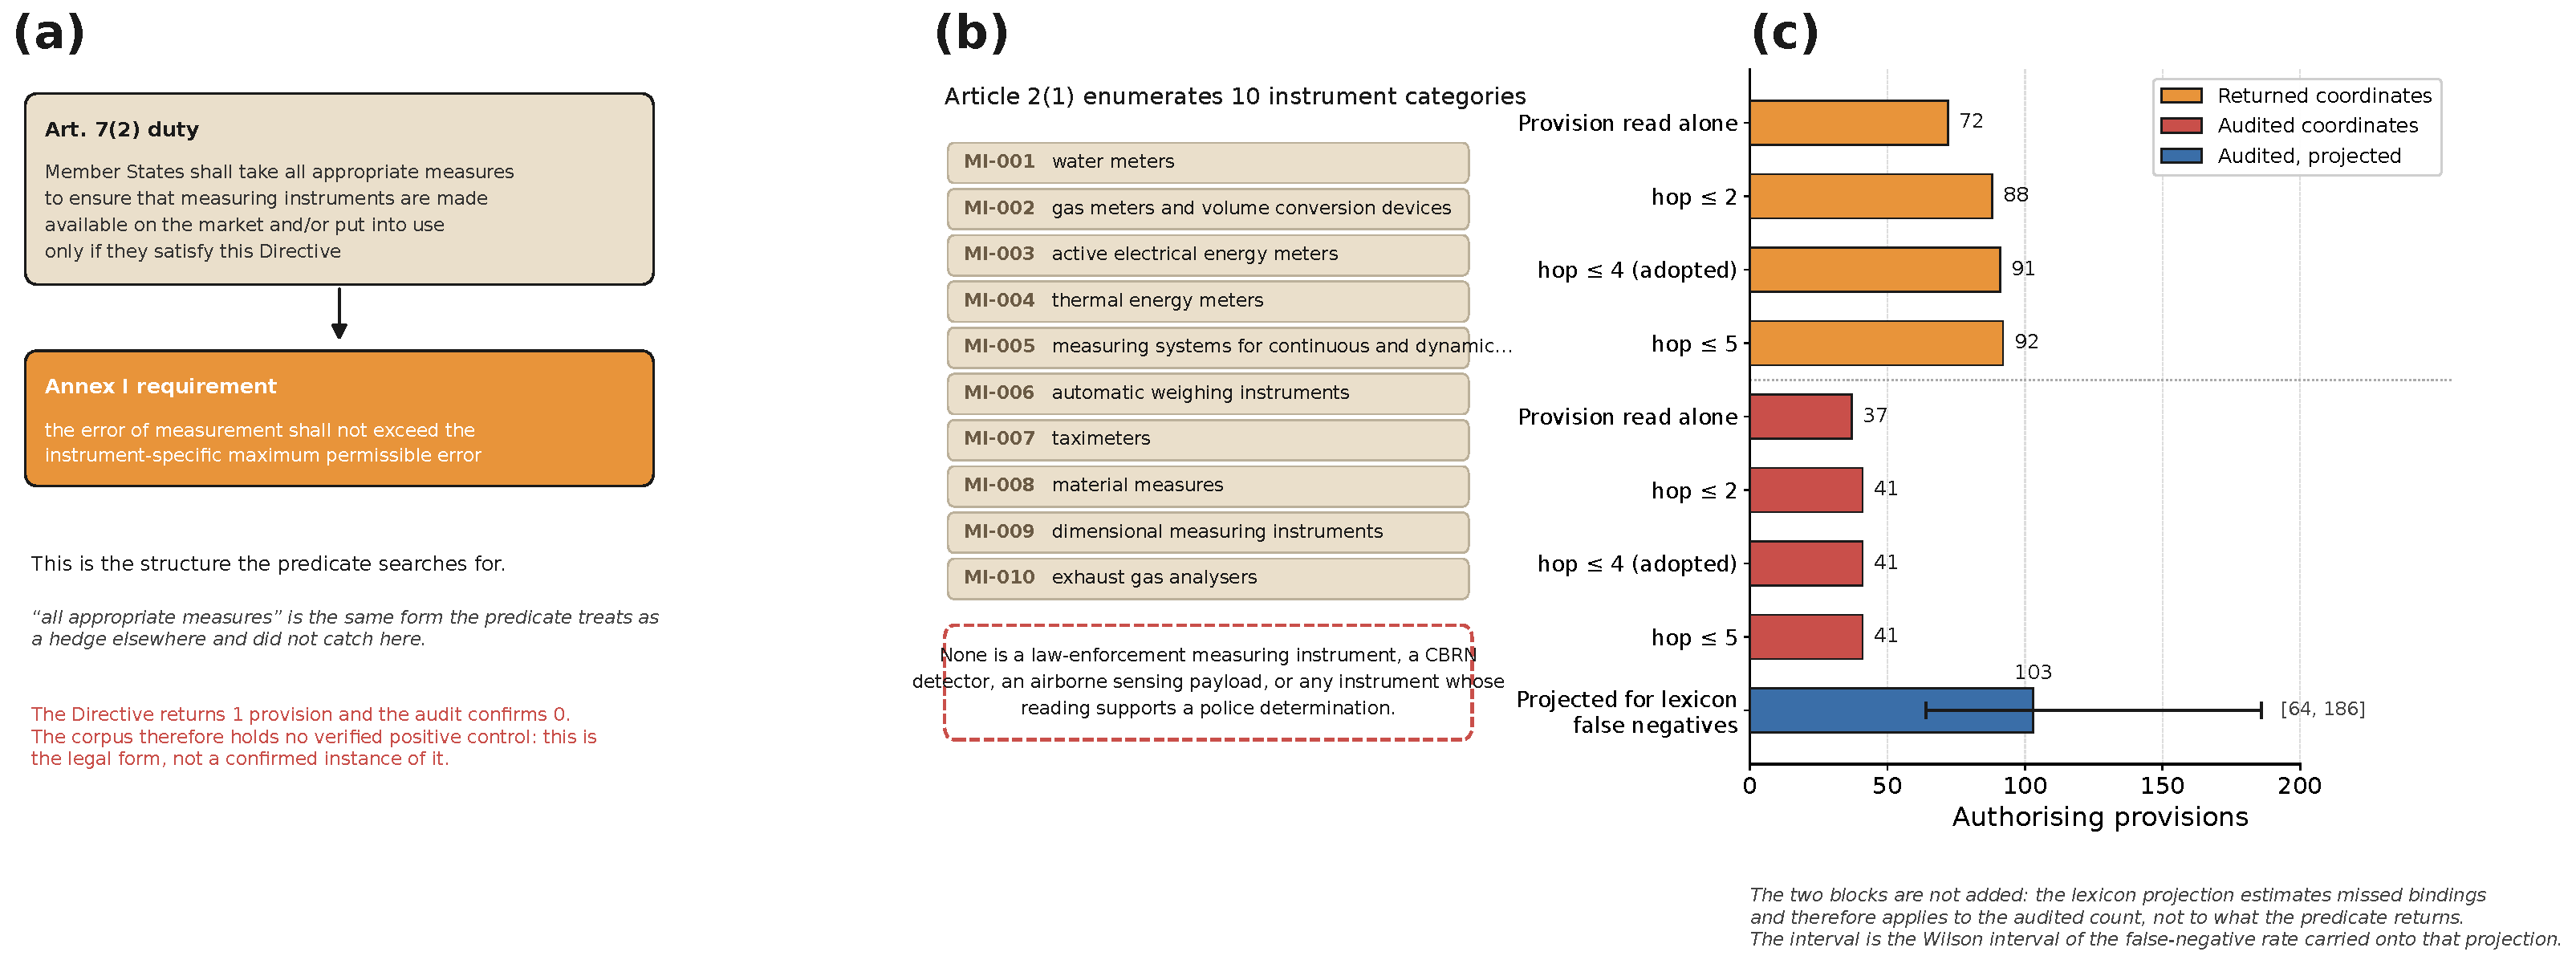
\includegraphics[width=\textwidth]{FigS}
\caption{The legal form that would bind sensing performance, its enumerated scope, and the robustness of the count. (a) The binding chain in Directive 2014/32/EU: Member States are to take all appropriate measures to ensure that instruments are made available on the market and/or put into use only if they satisfy the Directive, whose Annex I requires that the error of measurement not exceed the instrument-specific maximum permissible error. This is the structure the predicate searches for. The qualification on the Member State duty is shown because it is the same form the predicate treats as a hedge elsewhere and did not catch here, as Section 3.5 records. The Directive's single returned provision is rejected by the audit of Section 2.7, so the corpus contains no verified positive control and the chain is shown as the legal form rather than as a confirmed instance of it. (b) Article 2(1) enumerates the ten instrument categories the Directive applies to. None is a law-enforcement measuring instrument, a chemical, biological, radiological or nuclear detector, an airborne sensing payload, or any instrument whose reading supports a police determination. The gap is not an immature legal form; it is a boundary that was drawn. (c) The count under each variant of the rules that produced it. The upper block is in returned coordinates and the lower block in audited coordinates; the two are not added, because the lexicon projection of Section 2.6 estimates missed bindings and therefore applies to the audited count of 34, not to the 91 the predicate returns. The interval on the last row is the Wilson 95\% interval of the false-negative rate carried onto that projection.}
\label{fig:f4}
\end{figure*}

claim that the sweep covered three languages described the pattern list rather than the evidence. Symmetrising the three languages is the repair, and it is the same repair the determinacy lexicon received at the v14 refreeze; that it was still needed here is reported in Section 4.6.

These patterns occur in 51 of the 5,758 nodes, of which 21 are in the metrology Directive and six are Korean or Japanese. Among the 1,014 authorising provisions they occur in 12, and none of the 12 is a provision the predicate returns: seven are tier 1 and five tier 0. The symmetrisation added six nodes and no authorising provision, so it widened the search without changing what the search found. Those six deserve saying plainly, because a reader could take them for Korean and Japanese evidence that the sweep now has. They are not. All six match the accuracy concept in a non-measurement sense: closing a door accurately, operating the steering and braking controls accurately, operating an outdoor delivery robot's controls accurately, keeping records accurately in two driving-school provisions, and recording an operating state accurately. None is a performance condition and none is an authorising provision. After symmetrisation the Korean and Japanese contribution to this sweep is still empty, and the sweep's evidence remains English. Read one by one, none conditions an authorisation on a measured performance. Three concern the supplementary metrology marking, where it is affixed and that a distributor must check it is present (Articles 11(2), 22(3) and 22(5) of Directive 2014/32/EU). Three are in Implementing Regulation (EU) 2019/947, where accurate and precise qualify the information an operator must supply or the position a geo-awareness function must use, not a permission. One is the phrase calibrated air speed in Regulation (EU) 2018/1139 Article 2(8), a unit of measurement inside an aircraft category threshold, and one is the definition of measurement uncertainties in Regulation (EU) 2019/945 Article 3(35). One requires the holder of a Confirmation of Identification to keep its information accurate (14 CFR \S{}89.130(d)), and one requires that AI-generated content be marked in a machine-readable and detectable form (AI Act Article 50(2)). The remaining two are Article 4(1) of the Law Enforcement Directive, which requires personal data to be accurate, and Article 13(3) of the AI Act, which is the only substantive candidate among authorising provisions and is treated next.

An earlier version of this paper described two of these as the definition of a conformity assessment body in Regulation (EU) 2019/945 Article 3(1) and the definition of legal metrological control in Directive 2014/32/EU Article 4(1). Both citations were wrong, and wrong for the same reason: the extractor held each definitions article whole, so the node identifier \texttt{art\_3.1} meant the article rather than its first definition. Article 3(1) of Regulation (EU) 2019/945 defines unmanned aircraft; conformity assessment body is Article 3(11). Article 4(1) of Directive 2014/32/EU defines measuring instrument; legal metrological control is Article 4(3). The repair reported in Section 2.10 splits those articles into their numbered definitions, which is why neither now appears among the authorising provisions at all.

Three of the 51 nodes fall in Part 89, and they are the reason this subsection no longer reads as a flat negative. One is \S{}89.130(d), listed above. The other two are \S{}\S{} 89.310(h) and 89.320(h), the message-element performance requirements, which state the only numeric performance thresholds the sweep finds anywhere in force on the police route: the reported geometric position accurate to within 100 feet with 95 per cent probability, the reported geometric altitude to within 15 or 150 feet on the same probability. Neither is an authorising provision, and neither is reached from \S{}89.110(b) by any edge in the graph, but \S{}89.110(b) reaches both by the textual chain of Section 3.4. The sweep therefore confirms, from an instrument independent of the predicate, both halves of this paper's finding: a stated performance threshold does condition an operating permission on the police route, and the property it governs is the aircraft's report of its own position rather than anything the aircraft senses about the world. No pattern in the sweep

matches a provision that conditions a permission on the accuracy of a chemical, biological, radiological, thermal, acoustic or visual determination, in any of the sixteen instruments, on either route.

Article 13(3) requires the provider to state, in the information accompanying a high-risk system, the level of accuracy against which the system has been tested, and the accuracy it points to is set by Article 15. Article 15 is therefore the strongest candidate anywhere in the corpus. It does not appear among the twelve because it is not an authorising provision, which is the first thing to say about it; the reason it fails on the merits is worth stating as well, because it is the reason the paper's whole construct is built the way it is. Article 15(1) provides that high-risk AI systems shall be designed and developed in such a way that they achieve an appropriate level of accuracy. The operator is mandatory. The standard is not: appropriate is the hedge the predicate is defined to catch, and Article 15(2) confirms the reading by charging the Commission with encouraging the development of the benchmarks and measurement methodologies by which such a level would be measured, which is a statement that they do not yet exist. Article 15(3) requires only that the levels and metrics be declared in the instructions for use, and Article 13(3)(b)(ii) carries that declaration into the information the provider supplies. None of Article 15(1) to (3) is an authorising provision at all: they impose design and disclosure duties on a provider and confer no permission, so they do not enter the population this paper measures, and Article 15(4) and (5), which do, reach no evaluation. The AI Act thus contains the vocabulary of measured performance, attached to a duty on a manufacturer and hedged, and does not attach it to the authorisation under which a police agency deploys the system.

Article 15 is not the only place a counterexample could be, and the conformity-assessment machinery of Article 43 has to be examined before the claim can be made for the instrument as a whole, because that is where a permission would be attached to an assessment if it were attached anywhere. Paragraphs (1) to (3), (5) and (6) are not authorising provisions on the predicate's reading: they direct a provider to a procedure rather than conferring a permission, and paragraph (1) hedges with may in any case. Paragraph (4) is an authorising provision and reaches tier 1, mandating a fresh assessment after a substantial modification without conditioning anything on a determinate operator. Paragraph (3) is the one that merits adjudication rather than a tier. It provides that where a listed act lets a manufacturer opt out of third-party assessment, that manufacturer may use that option only if it has applied the harmonised standards and common specifications covering the requirements of Chapter III Section 2. The predicate does not return it, because may use that option is not in the authorising lexicon; adding that phrase is a one-line change whose measured effect is to return Article 43(3) at tier 2 and move the returned count from 91 to 92. We report the omission rather than repair it, and the reason is that the provision fails the audit on its merits in a way that is worth more than the count. Conditions (i) and (ii) hold: a permission is conferred and a determinate operator conditions it. Condition (iii) fails, and it fails twice over. What only if conditions is the application of harmonised standards, which is a declaration about process rather than a named evaluation procedure; and the assessment named in the same sentence is the one the manufacturer is permitted to opt out of. The strongest determinate conditioning of a permission in the AI Act therefore conditions the avoidance of an assessment, not the passing of one.

What lies behind Article 43 reinforces this, and it is a legal reading rather than a measurement, because the annex truncation described below removes it from the corpus. Article 43(2) routes the high-risk systems of points 2 to 8 of Annex III to the conformity assessment procedure based on internal control in Annex VI, and says in terms that this procedure does not provide for the involvement of a notified body. Point 6 of Annex III is law enforcement. Annex VI, 1,211

characters in the published text, defines that procedure as three acts of the provider upon its own system: it verifies its quality management system against Article 17, examines its own technical documentation against the essential requirements, and verifies that its design and post-market monitoring are consistent with that documentation. No performance threshold appears in it. The route by which a law-enforcement AI system reaches the market under the AI Act is therefore provider self-verification against a standard that Article 15 leaves hedged, with no third party and no stated metric. This is the same structure the paper reports for the police route in aviation and on the ground, reached independently and in the instrument that was the likeliest place to find the opposite.

This is the bound we can offer on the negative claim that the lexicon projection cannot, and it is narrower than it first appears, in two ways we should state. A binding may reach a performance threshold without naming one, by requiring a conformity assessment that delegates the threshold to a referenced standard, and that is the dominant form among the 23 aviation bindings we do count; the sweep would not see such a provision unless the delegating text itself used a performance term, and \S{}89.110(b) is an instance of exactly that: the sweep matches the threshold node but not the authorising provision that reaches it. Annexes are truncated at 6,000 characters, so the pages where thresholds are actually tabulated, including the instrument-specific tables of the metrology Directive, are largely outside the text the sweep reads. What the sweep therefore establishes is the absence of a provision that states a sensing performance condition anywhere in the corpus, authorising or not, not the absence of one that reaches such a condition by delegation. Within that scope it is a real bound, and a narrower opening than the 23 to 145 missed bindings of any kind that Section 2.6 projects.

\subsection{The result survives the choices that could have produced it}\label{sec:3.7}

Path bound. Returned counts saturate at four hops; the fifth adds one across the corpus, and removing the unnumbered structural and chapter edges entirely changes the count from 91 to 89 (Table 2). Audited counts saturate earlier, at two hops (Table 7). The bound was frozen before the audit and is not revised in the light of it, but the audited column shows that relaxing it past two hops buys no binding and costs precision at every step.

Scope restriction. A constraint derived from one mission may only match instruments in that mission's domains. This was the most outcome-determining discretionary choice in the earlier design, and it is worth saying what became of it: the restriction operates only where a constraint is matched to instruments, and no quantity reported in this paper passes through that step. The predicate runs over all 1,014 authorising provisions in all sixteen instruments regardless of which mission motivated the study, so the domain rates, the path variants, the carve-out comparison and the audit are unaffected by it. Reporting its effect would require the constraint-level counts that Section 3.8 withdraws, so we do not report one.

Hedge rule. A path is capped when any node on it carries a hedge. Because nodes are paragraphs, a paragraph in which a determinate condition and a hedge govern different clauses is capped even though the condition stands, and this can only remove bindings, so it biases towards our own conclusion. Removing the cap entirely, the most generous variant the rule admits, raises the returned count corpus-wide from 91 to 116 (Fig. 4c). An earlier version of this paper added that the 25 new returns contribute no audited binding. That statement is withdrawn as a sensitivity result, because it is true by construction rather than by measurement: the audit population is the 91 returns of the adopted rule, so none of the 25 carries a label and none could have been counted as a binding. What the row establishes is the size of the returned set under the most generous

reading of the hedge rule, and it is silent on how many of those returns would survive an audit. The same applies to the hop $\le$ 5 row, whose single additional return is likewise unlabelled.

Lexicon. The validated false-negative rate in the tier-1 population is 12.6\% [4.7, 29.5], and none of the observed false negatives concerns sensing or measurement performance (Section 2.6). Two statements an earlier version made about that rate are withdrawn. It is not a ceiling on the instrument's miss rate but a floor, because the validation samples only tier 1. Tier 0 was sampled separately and later (Section 2.10), and what it returned was not a missed binding of the kind the validation looks for but a missing class of lexicon terms; repairing that moved four Japanese provisions from tier 0 into the audited set, which is itself a measurement of how much the tier-1 rate understates the whole. And the absence of a language penalty is not shown: English returns 2 of 12 against 2 of 22 for Korean and Japanese together, Fisher exact p = 0.60, and a simulation puts the power of that comparison at 0.07 against a non-English rate of 30 per cent. That is an absence of power, which Section 3.3 refuses to read as equivalence elsewhere, and we refuse it here. The rate is a floor on the instrument and it is a low one: carried onto the audited counts it implies a recall near a third corpus-wide and far lower on the police route (Section 3.4). Separately, the lexicon contained a defect that no sensitivity in this list would have caught, because it suppressed a construction rather than mis-scoring one; it was found by testing the paper's own defeater and is reported with its effect in Section 2.10.

Corpus composition. The two instruments added after freezing are the two most likely to refute the paper. Both are reported above and neither refutes it. We no longer claim, as we did, that the metrology directive supplies a positive control demonstrating that the predicate finds the structure when it is present: its one returned provision is rejected by the audit, and the corpus therefore contains no verified positive control. This is a weakness of the instrument and we state it as one.

Audit. Precision is 0.451 [0.352, 0.553] over the returned set and differs by domain (Section 2.7). Every returned provision was labelled in two passes by one investigator using a language model as the instrument, so what the agreement figures measure is repeatability of the procedure and not agreement between readers. Agreement over all 74 labelled records is 51, $\kappa$ = 0.448 against a marginal ceiling of $\kappa$max = 0.520, with Gwet's AC1 at 0.577; outside the single ambiguous sentence pattern agreement is 51 of 56, which is the residue after the disputed cell is deleted and estimates nothing. Those 74 are the records both passes saw. One of them left the returned set under the lexicon symmetrisation of Section 2.10, and 18 records entered it after the passes were complete, so the agreement figures describe 74 records of which 73 are in the current returned set of 91 and none of the 18 later entrants is included. The audit was performed after the ruleset was frozen and no rule was changed in response to it.

Denominator. The authorising population is itself audited at 0.494 [0.386, 0.602] and the contamination is uneven, heaviest among the cross-cutting instruments (Section 2.8). Every rate is therefore reported in both coordinates. Correcting the denominator moves every rate upward and widens the aviation-to-ground contrast, so the nominal pair is the conservative one and no conclusion turns on the choice.

Determinism. The adjudication re-runs bit-identically from the frozen ruleset across hash seeds, and the corpus files verify against their recorded hashes.

\subsection{Why constraint-level counts are not reported}\label{sec:3.8}

The earlier design of this study reported outcomes for each of the 63 derived constraints. Doing so requires translating each constraint into search terms for four legal systems, and that

step is performed by a person rather than by the predicate. We tested whether it is reproducible. Twelve constraints were drawn at random, and the constraint sentences, the corpus and the termwriting rules were given, with nothing else, to a second term-writing pass made without access to our term lists, our results or this manuscript. The pass was executed by the same investigator using a large language model, so it measures the stability of the step under re-execution from the written rules rather than agreement between two people; it is the weaker of the two readings, and the result is poor under either. Applying the re-written terms through the same adjudicator reproduced our outcome class for 5 of 12 constraints. The outcome class takes four values, which are the ones the adjudicator can return: no concept reached, no determinate binding, not an authorising provision, and determinate binding. Our register produced 8, 3, 1 and 0 of them; the re-written register produced 3, 5, 2 and 2. On that scale Cohen's $\kappa$ is 0.184, with po = 0.417 and pe = 0.285. The full cross-tabulation is in Table 10, and we give it because a $\kappa$ on 12 cases and four classes is not interpretable without one: the number is reported as evidence that the step is unreliable, not as an estimate of how unreliable.

\begin{table}[!htb]
\centering
\caption{Outcome classes for the twelve held-out constraints, our register against the blind re-written register. Agreement is the diagonal, 5 of 12. Blind re-written register}
\label{tab:t10}
\small
\begin{tabular}{@{}lrrrr@{}}
\toprule
Our register & No concept & No binding & Not authorising & Binding \\
\midrule
No concept reached & 3 & 2 & 2 & 1 \\
No determinate binding & 0 & 2 & 0 & 1 \\
Not an authorising provision & 0 & 1 & 0 & 0 \\
Determinate binding & 0 & 0 & 0 & 0 \\
\bottomrule
\end{tabular}
\end{table}

The disagreements are instructive and symmetric. The re-written terms returned a determinate binding in two places where ours did not. The first is the headline constraint of the earlier design, which we had scored as reaching no determinate path; inspection shows the match is an artificial-intelligence classification provision reached through generic terms. The second is a constraint for which our terms returned no match at all while the re-written terms returned sixteen; inspection shows those sixteen to be driving-licence surrender provisions in the Japanese and Korean road-traffic law, matched through a grammatical particle. Neither register dominates: both produce false positives, in different places, and the re-written register produces them in the direction that would refute this paper.

We therefore report no constraint-level counts in this paper. The constraint registers are published because they document what the missions demand and are reusable, but the measurements above are confined to quantities that no analyst-written search term enters: the domain rates in Tables 9 and 8, the path contribution, the carve-out comparison, and the scope of the metrology Directive. This is a reduction in what we claim relative to the earlier design, and it is the reduction the reliability measurement requires.
